\documentclass[conference]{IEEEtran}

\usepackage{graphicx}
\usepackage{mathtools}
\usepackage{framed}
\usepackage{cleveref}

\begin{document}
\title{Projecting Global Filesystems into Local Containers for High-throughput Computing on HPC Resources}

\if 0

Abstract

Intro
- CVMFS & HEP applications
- NERSC/HPC resources
- mismatch, new requirements on HPC

Background and Challenges
- CVMFS requirements
- no FUSE, sudo, etc. on HPC
- Frequent updates to CMVFS
- need for past versions and present
- version consistency issues/mismatch with shared filesystem semantics
- DVMFS

-------------------

Identifying Dependencies
- tracing vs. static analysis
- represent deps. as a set of files -> equivalence between the two approaches
- possibility to include more than requested
- WLCG as testbed for tracing
- overhead of tracing
- sampling ratio for live applications

Projecting a Global FS
- projections vs. images
- SquashFS images vs. Docker, ...
- Shrinkwrap
- quantify image size vs. projection size
- data, metadata, cache costs
- creation costs

--------------------

Managing CVMFS Containers at an HPC Site
- multiple snapshots at different versions
- cost of large number of container images (storage, distribution, etc.)
- extreme cases: massive NERSC image vs. loads of tiny containers
- possibility of replacing an image with an augmented version to serve 2 apps
- tradeoffs in space, creation time, etc.
- online problem: create vs. augment

---------------------

PoC Implementation
- consider (path, ID) to deal with versions
- Jacard distance metric
- group images with common parts
- fast to (approximately) compute
- putting too many disjoint pieces in an image pushes it farther and farther away
- LRU to clean up

Evaluation
- sample workloads
- image vs. projection vs. cache size
- space savings
- image re-use
- construction time
- choice of alpha

----------------------

Conclusion

\fi

\author{
\IEEEauthorblockN{Nicholas Hazekamp}
\IEEEauthorblockA{University of Notre Dame \\
Notre Dame, Indiana 46556 \\
nhazekam@nd.edu}
\and
\IEEEauthorblockN{Tim Shaffer}
\IEEEauthorblockA{University of Notre Dame \\
Notre Dame, Indiana 46556 \\
tshaffe1@nd.edu}
\and
\IEEEauthorblockN{Jakob Blomer}
\IEEEauthorblockN{\&}
\IEEEauthorblockN{P. Samuel M. Teuber}
\and
\IEEEauthorblockN{Douglas Thain}
\IEEEauthorblockA{University of Notre Dame \\
Notre Dame, Indiana 46556 \\
dthain@nd.edu}
}


\maketitle

\begin{abstract}
High energy physics research at CERN has a large and rapidly growing need for computation.
To bridge the gap, may scientists are looking to HPC resources.
HPC environments provides a platform for large
batch computation, similar to the WLCG.
However, the restrictions on computation,
such as limited internet access and prohibiting FUSE,
clash with HEP's reliance on CVMFS as global filesystem
for software.
As most LHC jobs uses 
only a small portion of CVMFS,
a more fine-grained approach to preparing container images 
is needed to limit creation time and storage.
Shrinkwrap introduces a method for creating and
updating projections, but a framework for managing
theses is needed.
...
\end{abstract}



\section{Introduction}

High energy physics research at CERN has a large and rapidly growing need for computation.
With upgrades to the LHC scheduled in the coming years,
the amount of computation required will increase dramatically.
The simulation and analysis workloads at CERN are primarily performed using software distributed
via the CernVM File System (CVMFS).
CMVFS provides a read-only, distributed file system using HTTP for network transport and extensive local
caching to rapidly distribute updates in software across the WLCG.
The Worldwide LHC Computing Grid (WLCG) currently satisfies most of the computational needs of the LHC experiments.
With the upcoming high luminosity upgrades to the LHC,
the computational resources needed will nearly double (?? check this) by 2026,
% On CERN's page it estimate 50-100X need, argonne had a report that was 10-20X
prompting researchers to turn to available high performance computing (HPC) resources to meet demand.

HPC environments provides a platform for large
batch computation, similar to the WLCG.
In contrast with the WLCG's single slot submissions,
HPC applications typically consist of parallel jobs using several cores up to a full machine for each submission.
Most HPC systems have site-specific configuration and security requirements.
These can take the form of limited network availability at computation nodes,
limited container support,
and restricted access to privileged system operations (such as FUSE).
These restrictions present challenges when porting CERN's HEP applications,
such as difficulties submitting tasks,
inability to access required software,
and additional time spent converting between image and container formats.

Dependence on CVMFS to distribute experiment software currently makes it impossible to take advantage of many HPC sites.
CVMFS requires unrestricted network access and is implemented as a FUSE module,
which sites often disallow for security and management reasons.
Some sites, such as NERSC,
have attempted workarounds for providing CVMFS,
such as creating large images containing all of the software stored in CVMFS (500GB-1TB) or
maintaining separate specialize systems for distributing 
CVMFS, such as DVMFS.
However, both of these existing solutions require 
hours to days of attention from system administrators to deploy or update,
which leads to lag between the available software and the current version.
Additionally for systems that utilize large container images, large amounts of storage are needed to maintain different versions.

Since each LHC experiment job uses 
only a relatively small portion of CVMFS,
a more fine-grained approach to preparing container images would reduce the time spent creating images and allow for more precise control of the software versions in use.
This could also reduce the storage required at each worker node and the network bandwidth spent transferring images.
We modified the reference implementation of CVMFS to allow us to capture the filesystem interactions of a live HEP applications.
Using this live tracing or static analysis,
we are able to determine exactly which parts of CVMFS must be included in a container image for a particular job.
We developed a tool, Shrinkwrap, that can \emph{project} CVMFS (or a subset thereof) at a particular version into a traditional filesystem.
Such a \emph{projection} of CVMFS is suitable for inclusion in a static container image that does not depend on FUSE or network access.

When providing CMVFS at an HPC site,
the cost of creating, distributing, and storing customized images for a large number of jobs and users imposes additional challenges.
The na\"{i}ve approach of creating a projection of CVMFS for each job results in significant computation, storage, and bandwidth overhead.
Acknowledging that jobs frequently have significant overlap in dependencies,
we propose a metric for determining the similarity between projections.
This gives the possibility of identifying existing container images that could be re-used to fulfill a new submission.
In addition, we explore the trade-offs in automatically augmenting existing projections to allow container images to support multiple distinct job types.
We bring these tools together to propose a potential enhancement to a batch scheduler for making online decisions about whether to create, reuse, or augment projections of CVMFS to efficiently support high-throughput HEP jobs on HPC resources. 

%TODO summarize results

\section{Background and Challenges}

\subsection{CVMFS}
The CernVM File System (CVMFS) is a globally distributed filesystem designed for providing efficient,
read-only access to scientific software.
CVMFS is primarily used for distribution of High Energy Physics (HEP) software used as part of the Large Hadron Collider (LHC) at CERN.
Researchers at CERN use CVMFS as the primary means of distributing the analysis and simulation software they develop to the Worldwide LHC Computing Grid (WLCG).

Each WLCG site commits to providing some fixed amount of computational resources for analyzing particle collision events and running simulations.
Worker nodes at each site must be configured to mount CVMFS as a prerequisite to performing any computational tasks.
Since CVMFS is implemented as a FUSE module,
WLCG sites are expected to support FUSE on their worker nodes.
CVMFS also relies on global configuration files,
requiring administrative involvement in preparing worker nodes for WLCG jobs.
In addition, sites generally provision some infrastructure to support CVMFS,
such as caching proxies to reduce load created by local workers on publicly accessible filesystem servers.

As a result, it is difficult to contribute computational resources toward the LHC experiments without making some site-wide provisioning and configuration changes.
This is not an issue for the WLCG sites,
as they provide dedicated computing resources and can customize their setups to meet the requirements of CVMFS.
For a professor attempting to harness a campus cluster,
on the other hand, these requirements present a serious barrier.
Parrot, a debugging tool and personal filesystem developed at the University of Notre Dame,
can be used in cases where privilege on the worker nodes is limited and FUSE is not available but still requires unrestricted network access.
For computing at scale, it is important to provide a caching proxy as well,
which is likely to require assistance from administrators.

\subsection{HPC}

With the rapidly increasing demands of the LHC experiments at CERN,
HPC resources are an appealing source of computing power to supplement the WLCG.
Leadership class machines such as Summit (?) will by themselves be able to perform a substantial portion of the work of the entire WLCG today.
Use of national-scale HPC resources across the United States and Europe such as XXX, YYY, ZZZ could be key in meeting the computational demands following the LHC's high-luminosity upgrade.

Unfortunately, HPC sites are generally more restrictive than the previously mentioned campus resources.
In addition to limited privilege on workers and lack of FUSE support,
HPC sites often impose restrictions on network activity,
including outbound firewalls preventing access to CVMFS.

The US collaboration of the ATLAS project is currently taking advantage of computing resources at various supercomputers in the United States including Cori at NERSC.
For the deployment of their software the \texttt{uncvmfs} utility is used to unpack entire CVMFS repositories into standalone images (usually in ext4 or squashfs format) which in turn can be used to build Shifter or Singularity images.
While these images can very well be scaled out onto a large number of nodes inside the NERSC infrastructure,
the image build process takes around 24 hours which makes it difficult to deploy up-to-date versions of the software on a regular basis.
As these images contain complete copies of everything in CVMFS,
each takes on the order of terabytes,
necessitating careful storage management.
In addition, the process requires administrators for image creation, deployment, and cleanup.
Currently, this approach is used in production on the ATLAS and CMS experiments.
As additional experiments want to take advantage of the resources at NERSC,
the administrative burden of managing multiple CVMFS images on multiple software versions increases accordingly.
For the experiments to use the same images (saving time and cost at NERSC),
multiple groups would have to come to agreement about a single common set of software versions to use and adjust their pipelines elsewhere.
Both solutions introduce new inconveniences and administrative burden.

More broadly, the use of static, manually managed container images breaks user assumptions about the operation of CVMFS.
When running jobs using CVMFS,
researchers can specify the version of each repo to use,
allowing precise control over software and dependencies.
Each experiment has its own policies and procedures for choosing a software version;
some may use bleeding-edge analysis software or another experiment may prefer older, stable versions.
CVMFS is able to provide multiple customized views of the global filesystem without incurring much additional cost.
CVMFS also supports some more exotic features,
such as symlink resolution controlled by environment variables.
CVMFS as a whole does not map well to the semantics of a traditional filesystem.
Projecting CVMFS into such a filesystem can capture at most a single, static version of a repo and must necessarily eliminate some features,
such as environment-based symlink resolution at runtime.

% https://indico.cern.ch/event/587955/contributions/2937411/attachments/1683156/2705423/WahidBhimji-CHEP18-NERSC.pdf
Another similar approach in use at NERSC is DVMFS.
Since creating static container images containing CVMFS is costly and difficult to customize,
DVMFS instead uses Cray DVS IO forwarders to mount a copy of CVMFS served over NFS.
This allows for less administrator involvement,
since the mirrored copy of CVMFS can be automatically updated on a regular basis.
After dealing with several implementation problems,
DVMFS is currently deployed at NERSC as an alternative to static images.
While this approach affords more flexibility in choice of repos and software versions,
it increases the job startup time and places additional requirements on the infrastructure.
To be usable in production, DVMFS requires a sufficient number of DVS servers to be provisioned.
DVMFS is nonetheless a viable solution as long as the costs of developing/maintaining the service and allocating infrastructure do not grow too high.

\section{File Specifications}

The first step in addressing the high footprint 
of CVMFS repositories is to provide accurate 
specifications of the files, libraries, and packages
needed for each experiment.
These file specifications can then be used when 
projecting CVMFS into realized filesystems.
In general, the ability to project global filesystems 
hinges on the clarity of the file specification.
File specifications can be derived from several
different sources, such as 
usage traces, static analysis, or package listings.
The end goal of any of these methods is to 
create a comprehensive list of needed files and structure.
The nature of global filesystems flexible behavior
further extends file specifications by requiring
not just the files and structure, but also what
version/revision was used to verify the contents as well.

\subsection{Creation of Specification}
File specifications can be created several ways,
with the obvious option being handwritten.
However, this quickly becomes unfeasible with
even a moderate number of requirements.
This leaves the need for an automate method to create
specifications.
The first method is to create a sample trace for your
jobs. 
Creating a trace from a sample job allows 
for a listing of actual files used, which
can be more accurate than handwritten listings.
As these jobs are typically on the order of thousands
to millions of jobs, sampling a small subset
can provide good software coverage with little
additional overhead. % the computation is still used
The burden of creating these traces is
dependant on the method used,
which could be an LD\_PRELOAD library,
using Parrot to track used files, % I think parrot was mentioned previously
or building the tracing in to the application.
As we will see later, we chose application
level tracing as it provides more context
for the use.

The second automated method is to use static
analysis for discover requirements.
This would allow the application to be analyzed
prior to running to determine what packages are
linked.
Static analysis can be done at several levels,
each providing different levels of control 
and flexibility.
This could be more language specific in the 
form of following import lines in python or
include lines in C.
The alternative is to use repository specific 
methods for setting up the environment,
such as bash scripts for pointing to correct 
software versions, or 
analyzing SCRAM\cite{DBLP:journals/corr/cs-OH-0306014} lines
to determine the configuration.
With either of these methods the issues
that arise come from bleeding edge or
experiment specific code that is not directly
handled by the configuration.
There is a significant mix between languages,
configurations methods, and software organization
practices even within a single repository,
which compounds the above issues in this method.

An combination of tracing and static analysis is the
use of package listings. 
Package listings provide a high level indication
of the software needed, and allow for 
flexibility on the specifying user about the
exact files needed.
Using high level packages provides a method
for handwritten/tuned specifications that 
include all aspects of the package.
The downside of using packages is that in
their flexible, forgiving specification
they can be bloated and include unnecessary
files and data.
Packages also require that there is consistent
software organization, which often differs
between repositories.

For the analysis and creation pipeline discussed
later in the paper, tracing was used to provide
the file specifications. 
Tracings flexibility between repositories
and more precises file inclusion allow
for a lean package that provides coverage for
an experiment.

\subsection{Trace Sampling}
Tracing was selected as it provides a consistent 
behavior between experiments and use cases.
This allows the solution to port between applications
quickly without having to delve in to the applications
specific configuration.
As previously mentioned, there are several methods for
obtaining a trace from a file.

Tracing was implemented in the CVMFS software and
interacts via the FUSE interface.
The tracing utility has been implemented in a way that 
minimizes the overhead if the tracer is deactivated and 
also minimizes the measurable overhead in the FUSE calls for an activated tracer 
by delegating the actual log writing to a separate thread to avoid blocks 
during the accesses to CVMFS. 
In fact, for a deactivated tracer the entire overhead consists of 
a single inline if for a subset of the FUSE calls.
This allows the actual observed CVMFS usage to  be tracked
and then used for determining the file specification.

Despite assumption that both CVMFS and FUSE will be limited
on the HPC site, this methods was used as it is reasonable to
allow for sampling of these jobs on WLCG. 
WLCG provides the flexibility of using CVMFS and FUSE, without
having to implement or provision a separate tracing infrastructure
at each site.
Additionally, as many of these jobs would have originally been 
destine to run on WLCG, the sampling sizes are unlikely to 
create significant overhead.
Using CVMFS for the tracing allows CVMFS's just-in-time deployment
of files to patch the environment and give an accurate view without
the risk of missing files.

Regardless of how the trace was produced,
there are several ways a trace needs to communicate 
which files and how they were used.
Below is a table describing different axes by which a 
specification can be tracked:
\begin{table}[h]
    \centering
    \begin{tabular}{|c|c|}
    \hline
    Number of files & The number of files in a given subtree. \\ \hline
    Depth of Tree & The largest number of nested directories. \\ \hline
    Width of Tree & The number of directory splits in a subtree.\\ \hline
    Size of files & Sum of the files contents in subtree.\\ \hline
    Actual files & The actual file names.\\ \hline
    Revision/Release Number & The version of subtree/compatibility. \\ \hline
    Checksum & The files computed checksum. \\ \hline
    File type & Directories vs Files.\\ \hline
    Usage type & File open/stat/directory listing.\\ \hline
    \end{tabular}
    \caption{Description of different axes in File specification distance}
    \label{tab:distance_axes}
\end{table}


\subsection{Defined Consistency}
In order for a file specification to accommodate 
the need for describing the structure and contents
the specification goes beyond a generic file listing.
A file specification needs to include enough information
to establish the directory structure and verify the contents.
This can be done in several ways, 
such as computing the checksum of contents,
using global revision numbers, 
or running verification software.
Computed checksums provide a system agnostic approach
to verification by allowing the checksum to be computed
at specification and verified before use.
Computed checksums provide a
consistency guarantee to the byte level,
but are often expensive at runtime for large
production systems.
This approach is alleviated in systems such as 
Git and CVMFS as the contents' checksums are 
computed at ingestion into the repository.
This method relies on the underlying system computing
and providing this information for verification.

The use of a global revision number provides a quick reference
on the state of the repository at the highest level.
Global revision numbers can instantly verify the expected
contents, but does not give evidence of compatibility between
revisions.
As the revision number if global, any change to the repository
is reflected in a change to the revision number, which means 
some software is compatible between revisions.
This method leaves much to be desired when using common stable
packages that change irregularly.

Aside from computing and checking the contents of the
repository or it's files, it is possible to verify the
software using experiment computation.
This is a common method used to testing software
and works equally when the target software provides
coverage of the features used by the application.
The difficulty here is in providing tests that
behave consistently, verify if computation is
incorrect, and cover the desired features.
Though it is possible for the submitting user
to provide test with coverage, application
developers have a better grasp of it usage
and how to provide coverage in testing.
An additional method is to run the application
on a determined site for initial results and
compare in the future for verification, but
this relies on deterministic code which is 
not always the assumption in HEP computing.

I AM NOT SURE WHICH WE WILL USE. WRAP THIS UP LATER.

\section{Realization of CVMFS Projection}



\subsection{Definition of Projection}

In the case of global filesystems,
every time the filesystem is used locally
the flexible global state has to be 
locked for that concrete use case.
In the case of CVMFS,
this includes specifying the date-time
or revision number of the repository.
This state is used to determine 
what the global filesystem's directory
structure and file contents are, 
allowing for future use of the same state.
CVMFS is able to flexibly move
between these revision using the FUSE module
to determine the structure and files and
relies on HTTP to pull any missing files.
However, with neither the HTTP access or
FUSE permissions, a method is needed to 
create and track realizations of this
state for future use.

We call these realizations of the global filesystem
projections.
A projection is a concrete filesystem that can be
mounted, loaded, or copied into an existing system.
Projections can then be used to run experiments
and analysis using the global filesystem without
the previously mentioned permissions.
Projections have been used with CVMFS before,
in the form of unCVMFS and rsync.
UnCVMFS is a utility that projects an entire
CVMFS repository, at a set revision, into the local
filesystem. 
UnCVMFS utilizes CVMFS's data/file separation
to deduplicate the underlying data, but requires
entire repositories to be projected.
When used with several repositories for large projects,
unCVMFS can easily consume 500GB for single projection.
As is often the case, different experiments/analyses 
require different revisions that may conflict.

Rsync allows for file lists to specify and download
subsets of CMVFS repositories, but because it
was designed for general filesystem synchronization
rsync flattens the files introducing duplicate data.
This direct representation of the file tree also
excludes the possibility of shared data repositories
between different projections.

% Probably need to mention that many applications assume
% CVMFS software is installed/mounted at /cvmfs

\begin{figure}[h]
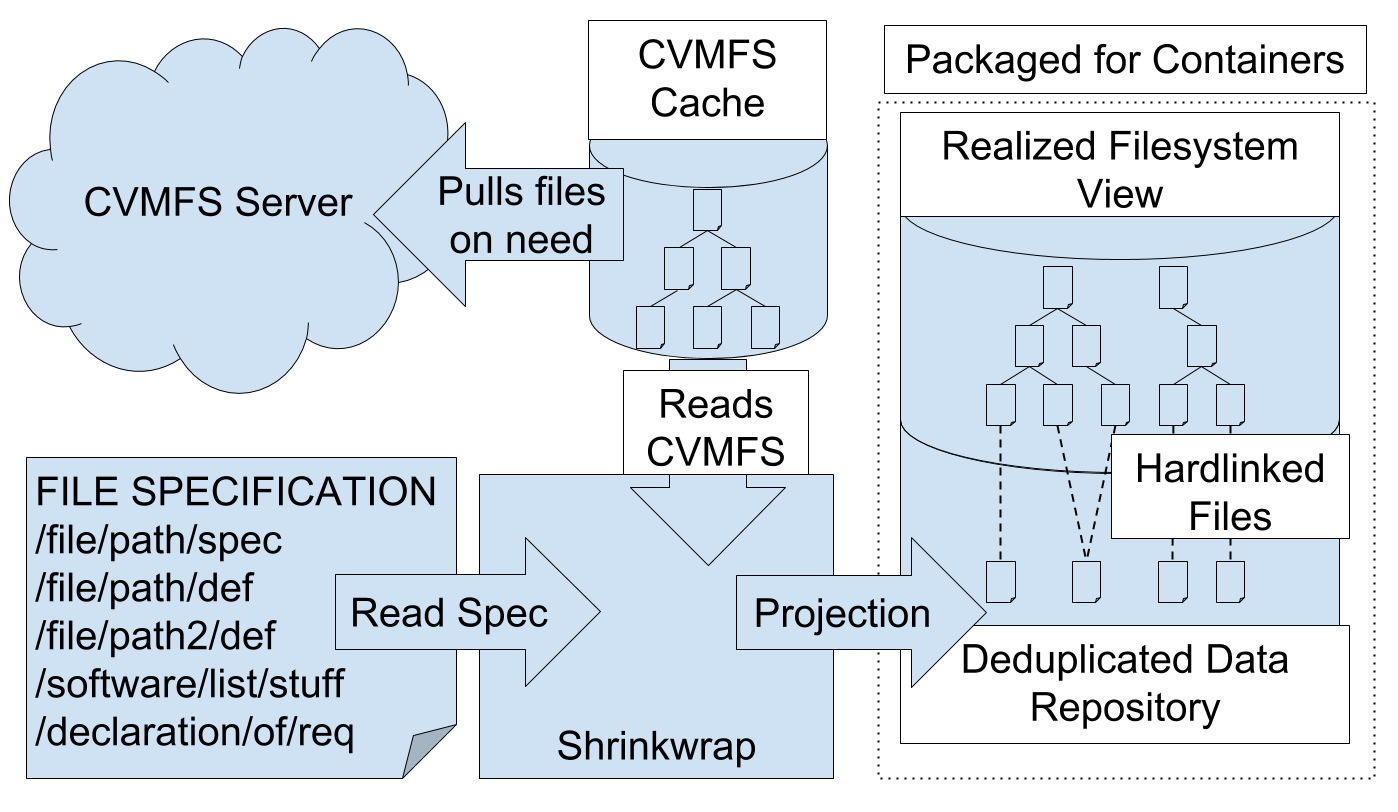
\includegraphics[width=\columnwidth]{drawings/shrinkwrap-structure.png}
\caption{Shrinkwrap Approach}
\label{figure:shrinkwrap-arch}
\end{figure}

We built the CVMFS Shrinkwrap utility,
a solution that leverages the best of both
unCVMFS and rsync.
Shrinkwrap uses the CVMFS's client interface to
create and update CVMFS projections.
Shrinkwrap uses a CVMFS configuration to specify the
revision of the repository, a file-specification list
to determine the repository subset to project, and
deduplicates the data in a user specified location.
Shrinkwrap can be configured to share the data
repository between several repositories and even
projections of the same repositories.
This allows for multiple realized projections
to coexist, with the desired projection
mounted for use.
In \Cref{figure:shrinkwrap-arch} you can see an outline
of the design of the Shrinkwrap utility.

These methods were compared to showcase Shrinkwraps
behavior and evaluate usage performance.
The first analysis compares all three methods pulling 
an entire repository, to allow comparision between the
three.
GRAPH OF DEDUPLICATED DATA/FULL REPO SIZE/TIME TO CREATE.
The second looks at the time to update existing repositories 
between verison.
GRAPH UPDATE TIME ON FULL REPO AND MAYBE SUB REPO(SUB REPO ONLY COMPARES RSYNC AND SHRINKWRAP)
The third looks at hosting several projection at once and
switching between them.
COMPARES RSYNC AND SHRINKWRAP. UNCVMFS CANT COMPETE.


\begin{figure}[h]
\caption{COMPARISON OF SHRINKWRAP unCMVFS and RSYNC}
\label{figure:projection-comp}
\end{figure}

\subsection{Packing Projections}

All of the above methods describe utilize CVMFS
and rely on the internet connection to create
the projections.
A core assumption of this paper is that internet
access is limited at the compute nodes, so a method
is needed to transform and use these projections
for computation.
For this we looked at several methods for providing
these projections and compared using 
Container images (images specific to Docker, Singularity, ect.)
versus SquashFS images.
The goal is to find a flexible, compatible intermediate
format that allows projections to be moved between sites
and technologies.
For this purpose, DOcker images, Singularity images, and 
SqaushFS are compared on their time to create,
storage requirements, and most importantly compatibility
with several used technologies, namely 
Docker, Singularity, and Shifter.

The first aspect is the creation of these images.
From a defined projection of a repository
what are the steps needed to create each of these image types.

GRAPH COMPARING BUILD TIME

GRAPH COMPARING STORAGE SPACE

TABLE COMPARING COMPATIBILITY AND SUPPORT

%MERGING PROJECTIONS

%INCOMPATIBLE PROJECTIONS
%It is often the case when using CVMFS
%an analysis job requires pieces of several repositories.
%As a result a method for merging and verifying that these
%repositories are compatible is needed.

When creating these images for analysis jobs its often the case that several
of these images may be created and used in the system.
Using Shrinkwrap to organize the repository data and projections,
the impact of an increasing number of images can be see in 
\Cref{figure:spec-size}.
This graph illustrates a new challenge that needs to be addressed.
As the number of experiments run and projections hosted by Shrinkwrap
increase. 
The raw number of images that need to be host increases to an unmanageable
size.
A solution is needed for how to manage these images and still
provide responsive execution of HEP analysis on HPC.

\begin{figure}[h]
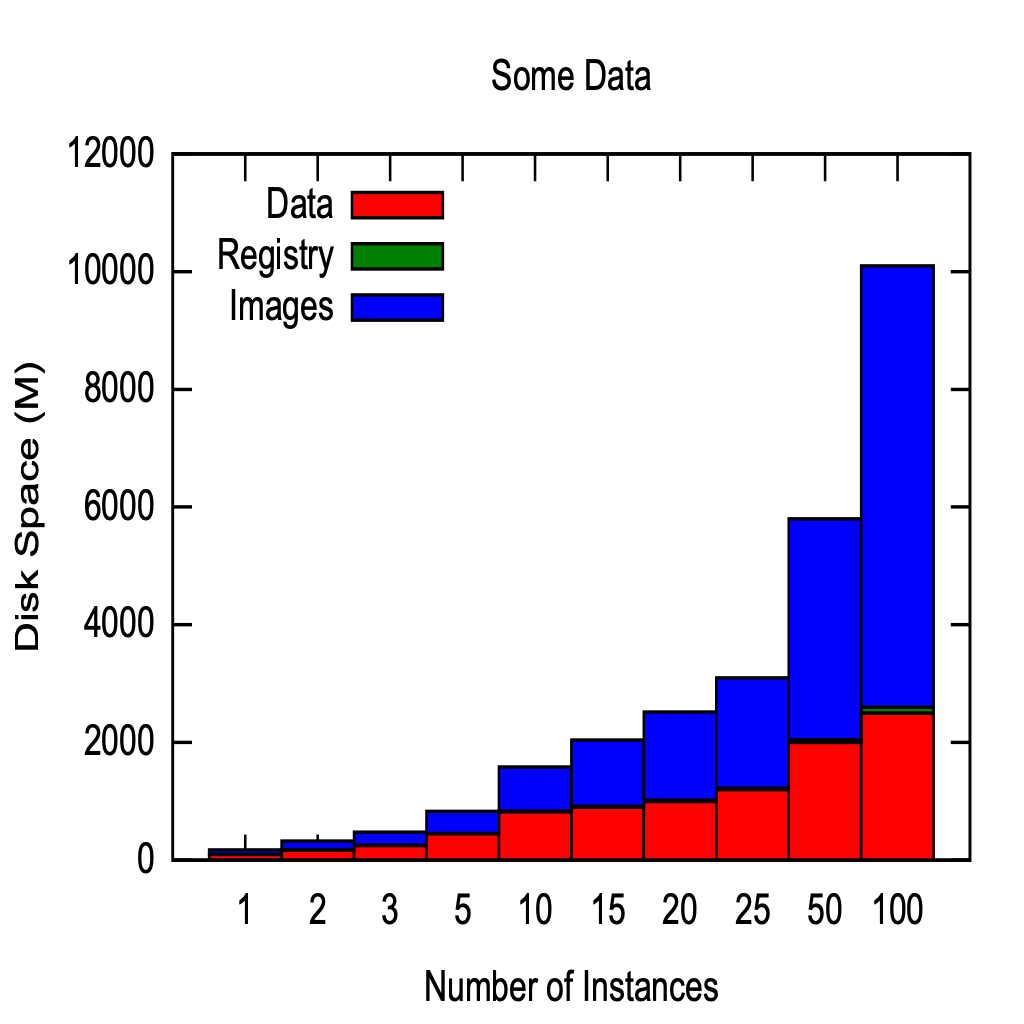
\includegraphics[width=\columnwidth]{plots/specification_size.png}
\caption{Additive effect of host many images.}
\label{figure:spec-size}
\end{figure}

\subsection{Use Cases}
Here we illustrate several real world use cases.
These use cases are being used as the existing solutions
were not feasible and a new approach was needed.
In analyzing these use cases we can see the beginnings of
the problem outlined in the previous subsection.

\subsubsection{Atlas at NERSC}

We are currently discussing options to integrate our shrinkwrap utility into the HPC deployment processes of ATLAS as we believe that the proposed software solution can help to reduce the overhead of HPC software delivery significantly. On the one hand the actual uncvmfs export process can be optimized as the current export workflow loads the entire CVMFS repository in a first step and later on removes certain files in the exported image which were not in fact needed. This is something that can be entirely avoided through the definition of exclusion rules passed to the shrinkwrap utility.

On the other hand, we believe that an export client which relies on the libcvmfs library might reduce the total overhead and therefore improve the export performance in comparison to both uncvmfs and rsync (for uncvmfs this is something that we haven’t had yet the chance to evaluate in an experiment).
As a longer-term goal, it might be useful to start tracing ATLAS simulation workflows on a few machines to collect data that might allow further export optimizations in a later stage through automated specification building.

\subsubsection{Benchmarking Containers}
For benchmarking purposes, the CERN IT-Department is interested in a ”Benchmark in a Container” solution which allows the distribution of standalone container images for system performance evaluations. For such benchmarks the IT-Department typically relies on simulation work- flows provided by CERN’s experiment collaborations. To execute these benchmarks in an easily portable and reproducible manner, it is of high interest to package these software workflows into containers. Since the workflows’ software stacks are usually stored inside CVMFS repositories, this is a perfect use case for the shrinkwrap utility and its Docker injection functionality.

For the image export the workflow’s resource-needs would be examined through the CVMFS tracing feature in a first step. This would then result in a log containing detailed insights on the paths which were accessed by the benchmarking workload. In a second step we can then produce a specification based on the tracing log which will allow an easy, efficient export of the necessary files from CVMFS. Afterwards the Docker injector can be used to inject the exported files into a prepared benchmarking container stored in a registry. Later, the same utility can be used to update the current container to an up-to-date software version or — depending on the exact use case — the utility could even be integrated into a continuous deployment mechanism which produces new benchmarking containers on every software update.

\section{Managing Projections as a Site-wide Resource}

A major queston not addressed by the Shrinkwrap tool is how to manage images after creation.
In the case of a small number of manually created container images,
this is not a serious problem.
Thus for integrating with the existing systems at NERSC,
Shrinkwrap alone might be sufficient.
We would also like to support CVMFS as a site-wide service,
e.g.\ with a batch system plugin that can automatically prepare container images on job submission.
This both minimizes direct administrator burden and more closely approximates user experience on other resources like the WLCG.
With static analysis and dynamic tracing of tasks,
we have ways to choose subsets of CVMFS to project to run specific tasks.
The user can collect this information themself,
or tracing, too, could be handled automatically.
We have seen two approaches to this in section ??.
If the same types of jobs are also run on other resources such as the WLCG,
it is possible to instrument a fraction of runs to build a profile of the type of task.
Alternatively, we could integrate tracing with image creation by automatically running exemplar tasks on the WLCG or on dedicated bridge nodes and collecting traces as necessary.
Assuming that accurate dependency information is available via some means,
we are interested in automatically providing suitable projections of CVMFS to users.

\subsection{An initial approach}

The simplest approach for automatically projecting container images is to create a suitable image on each batch job submission.
Unfortunately, this solution is very wasteful of computing time.
The average simulation or analysis job runs for XXX seconds,
while preparing an image for it using Shrinkwrap and mksquashfs takes on average YYY seconds.
This image creation is a serial step that must be completed before any actual processing occurs.
In addition, freshly created images must be transferred and stored on any nodes that will use them,
increasing load on the network and storage infrastructure.

The first step toward improving performance is to re-use previously created container images.
A single experiment submitting computational tasks is likely to request the same projection of CVMFS,
at least for jobs submitted around the same time.
It is straightforward to check for exact equality between projections as long as the system retains the set of files that went into their creation.
In particular, it is important to retain both the paths and the hash of the file contents or some other unique identifier.
This ensures that multiple versions of the same file are recognized as distinct entities.

Next, worker nodes need to be able to cache previously used container images.
Technologies like Docker currently operate this way (often to the chagrin of users and administrators doing scientific computing).
Since projections of CVMFS can be re-created on demand,
there is no need to carefully track which container images to keep.
For our evaluation,
we chose LRU as a simple caching policy.
Worker nodes are assumed to have some fixed amount of storage available for caching images.
Node-local scratch storage is sufficient for temporarily caching these images.
We also assumed that durable storage is available on the bridge machine for storing the data cache and projections associated with Shrinkwrap,
as well as a cache of container images derived from these projections.
Again, we chose LRU as a caching policy for our evaluation,
though administrators would be free to experiment with different policies.

Under this design,
on job submission the bridge machine first checks if the same projection had been requested before.
If so, it arranges to transfer its cached container image to worker nodes that lack that image locally.
If the bridge node does not have that projection built already,
it uses Shrinkwrap to create the requested projection,
then invokes mksquashfs to create the container image.
Once the bridge node places the newly created image in its cache,
the process proceeds as in the previous case.
The architecture of this initial approach is shown in figure ???.

\subsection{Evaluation of the Initial Approach}

We wanted to evaluate the viability of the simple design discussed in the previous section,
so we analyzed of a stream of actual job submissions to the WLCG.
Figure ?? gives a summary of the results.
We observed that for a single experiment at a given point in time,
the requested projection is fairly stable.
However, updates to software sometimes overlapped with previous job submissions,
leading to multiple projected versions of repos at the same time.
In addition, submissions from different experiments generally request different versions of repos.
Thus for a site servicing only a single LHC experiment and with ample storage for caching images,
the simple approach outlined above is sufficient.
For a more diverse workload like that of the WLCG,
however, the amount of resources spent creating and storing projected images rapidly increases.

This presents a problem for sites attempting to significantly augment existing computational capacity,
as they must be able to efficiently support jobs that vary widely both across experiment and time.
Since NERSC was willing to devote QQ~TB of storage to complete copies of CVMFS for their current container images,
the storage cost may be bearable.
It is not safe to assume,
however, that this will generally be the case.
Thus we need to find a way to more efficiently handle and store images while still retaining the flexibility of fine-grained per-job customization.

It is important to note that while the cumulative size of the generated container images grows quickly,
the projections themselves take up much less space.
This is due to the deduplication feature of the Shrinkwrap tool.
When creating a projection,
Shrinkwrap fetches any missing file data and stores it in a common content-addressable cache directory.
Shrinkwrap then hard links into the data cache to create the projection.
This allows multiple projections with contents in common to share their underlying storage.
Thus even with a large number of projections,
as long as the differences between projections are small the storage space required is modest.
When creating container images,
however, this deduplication is broken as it is not possible to share components between disk images.
When creating each image all data in the projection must be copied in.
We observed that the overlap between images was in many cases quite large.
We therefore investigated strategies for deduplication between static disk images,
as this would greatly reduce the storage and transfer overhead observed here.

\subsection{Quantifying Similarity between Projections}

Because of the difficulties in applying normal data deduplication across multiple disk images,
we developed an optimization strategy using additional knowledge about the behavior of CVMFS.
To better understand the overlap and similarity between projections,
we sought to quantify the degree to which two projections are related.
This would allow us to identify projections that are ``close'' (for some definition of close) as candidates for optimization.
We chose the Jaccard distance for this metric because it has a number of useful properties.
First, it is very simple to compute and operates on general sets.
For two sets $A$ and $B$,
the Jaccard distance $d_j$ is defined as follows.
\[
d_j(A, B) = \frac{|A \cup B| - |A \cap B|}{|A \cup B|}
\]
Second, there exist approximations such as MinHash that can quickly estimate the Jaccard distance between two sets.
Third, the Jaccard distance is a metric in the mathematical sense,
making it easier to reason about distances.
For the purposes of comparisons,
we represent a projection as a set of files in CVMFS.
It is not sufficient to represent a file solely by its path,
as different versions of a repo can have different data at the same path over time.
Therefore we represent each file as a tuple consisting of (path, hash) where the path is the absolute path of the file and the hash is a unique, content based identifier.
CVMFS already stores files by the hashes of their contents,
so this information is readily available.

For this application in particular,
the Jaccard distance captures several desirable properties of projections.
In the case of two projections that differ only by one file,
the Jaccard distance will be small.
Likewise for a par of projections with nothing in common,
the distance will be high.
And since the Jaccard distance is a proper metric,
we can find clusters of related projections;
If two projections are both found to be extremely close to a third projection,
we can conclude that the two are themselves close by the triangle inequality.

\subsection{Image Management as an Online Problem}

\begin{figure*}[t]
\centering
\fbox{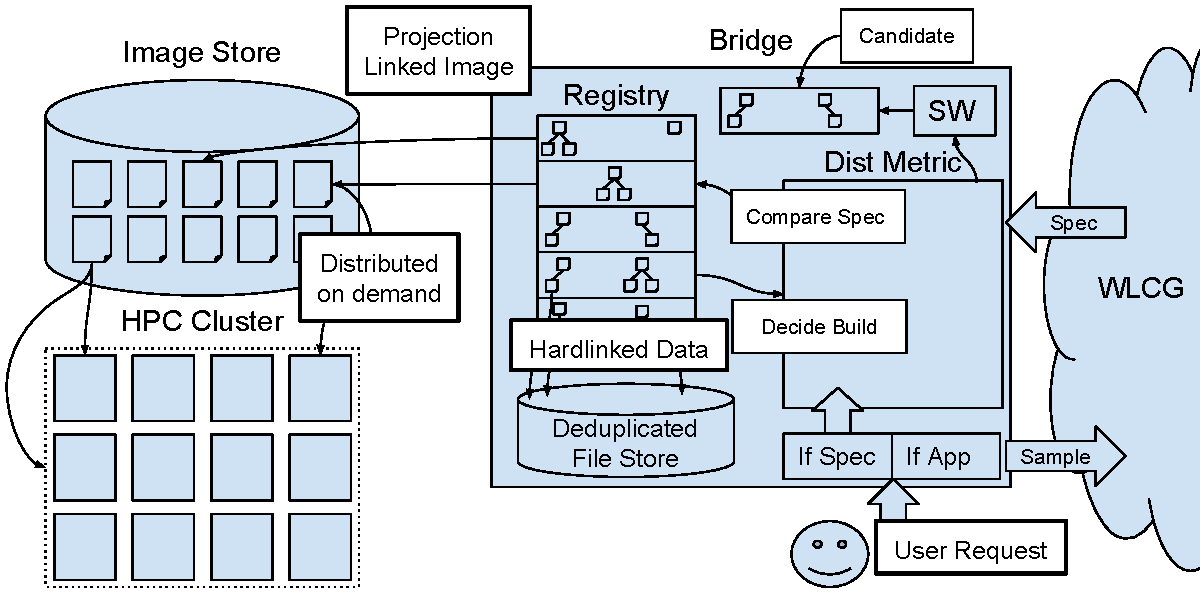
\includegraphics[width=0.95\textwidth]{drawings/system_architecture.pdf}}
\caption{System Architecture}
\label{figure:sys-arch}
\end{figure*}

Combining the tools and techniques introduced so far,
we are now ready to address the central problem in managing projected images as a site-wide service.
Rather than relying on administrators to manually manage images,
we must define a method for making a decision online as to how to efficiently satisfy the dependency requirements for batch jobs.
Our method must be suitable for inclusion as part of the setup for batch job scheduling and must be efficient in terms of both computation time and storage space.
We will extend the initial implementation discussed in section ?? by tracking distances between projections and allowing existing images to be augmented rather than creating new ones for each request.
\Cref{figure:sys-arch} gives an overview of the structure of this system.

Upon receiving a request for a projection,
we first hash the new projection according to the MinHash algorithm.
We always store the hash values computed for every projection we build to allow for fast clustering.
Next, we use MinHash to approximate the Jaccard distance between the new projection and all projections previously built.
Since comparisons using MinHash take constant time for a given probability bound independent of the size of the sets involved,
we can quickly identify cached projections that are similar to the new request.

To decide if two projections are ``close'',
we define the parameter $\alpha$ as the maximal Jaccard distance between closely related projections.
Since Jaccard distance is by definition between zero and one,
$\alpha$ must be in the same range.
Choice of $\alpha$ is left to the system administrators.
Very small choices of $\alpha$ require that projections be extremely close before considering them for merging.
In the extreme case with $\alpha = 0$,
only \emph{identical} images will be considered close so no images will be merged.
This results in a larger number of independent images.
Choosing $\alpha$ to be larger makes it more likely for images to be considered similar and merged.
This results in more augmented images that serve multiple tasks.
In the extreme case of $\alpha = 1$,
\emph{every} pair of images is considered close and merged if possible.
This results in large container images that have accumulated many projections.
We explore tradeoffs when choosing $\alpha$ and give recommendations based on observed patterns of activity in section ??.

Having selected a set of candidate projections that are close enough to the new request,
we next check each in turn to find either a superset of the requested projection or one without version incompatibilities.
In the case of finding a superset,
we can simply use the corresponding cached container image.
Presumably this superset was created by the merging process below,
so we are done.
Otherwise, we continue to look for a compatible projection
As discussed in section ??,
two projections are incompatible if they both include the same path but point to different data.
This situation can arise if for example a library in CVMFS is updated in place.
Old and new projections would include an identical filesystem path,
but the new version would have different contents.
This situation can arise in more subtle ways,
for example with symlinks controlled by environment variables.
Since projections of CVMFS must statically resolve such links,
incompatibilities can arise despite paths appearing compatible under CVMFS.
And candidate projections that are incompatible with the new request are removed from further consideration.

If no compatible projections were found among the candidates,
we create a container image for the projection as requested and add it to the cache.
Otherwise, on finding a compatible cached projection the next step is to augment it with the contents of the new request.
As previously discussed,
Shrinkwrap can update a projection that was previously created;
since we keep the projection used to generate each container image in the cache,
we can simply augment the selected projection with the new files from the request.
Next, we build a container image based on the newly updated projection.
The computational cost of this step could become high since we are creating larger combined projections.
Appropriate choice of $\alpha$, however,
bounds the distance between the combined projections such that the cost of creating the augmented container is arbitrarily close to cost of simply fulfilling the original request.
Since the augmented projection is the union of two different projections,
we can substitute it for both.
The container image for the augmented projection can replace the previous image,
so that the net increase in storage space comes only from the newly added files.
Since a single augmented image now serves two different batch job submissions,
we avoid making two copies of the common files and data.
In section ?? we explore the storage and computational costs of this approach in a more concrete setting.

\section{Evaluation}

\begin{table}
\centering
% not factually accurate...
\begin{tabular}{c c}
CPU & Xeon something 2 \\
Cores & 12 \\
Memory & 24 GB \\
Disk & 1 TB \\
Image cache & 32 GB \\
\end{tabular}
\caption{Description of each of the 24 worker nodes}
\label{tab:exp-setup}
\end{table}

\begin{figure}
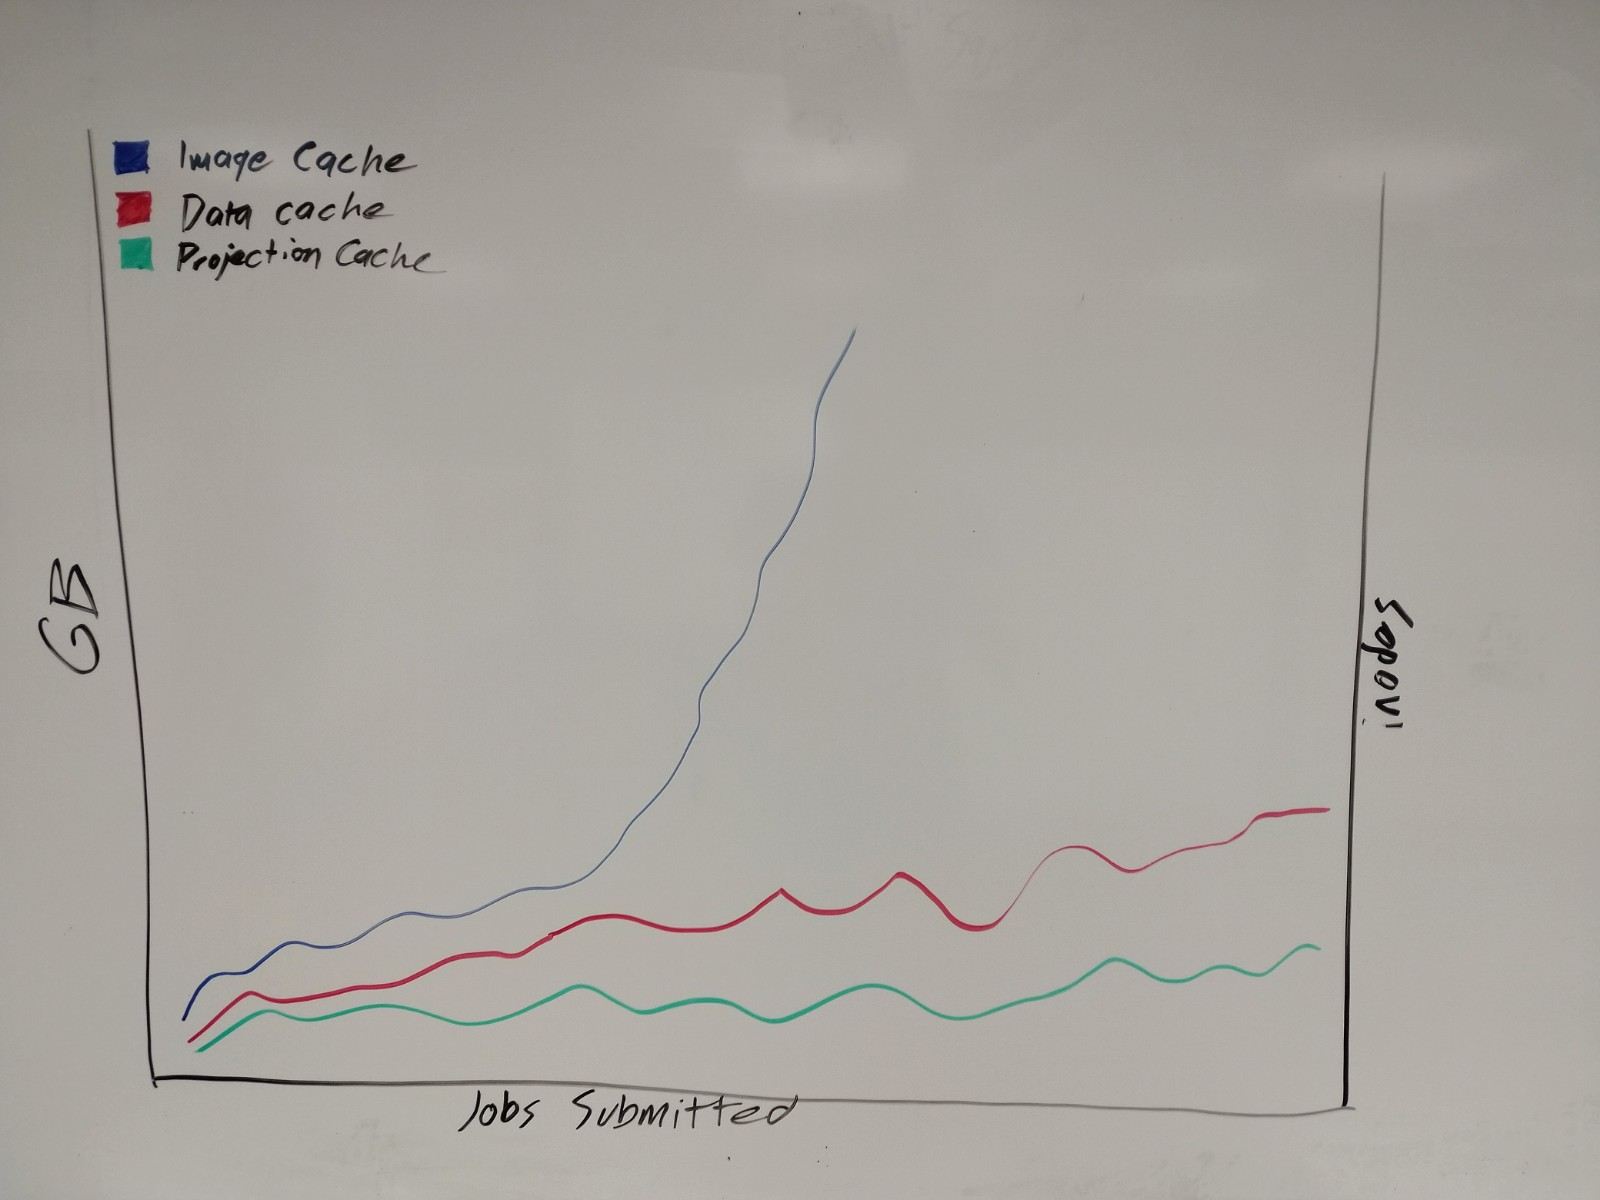
\includegraphics[width=\linewidth]{plots/IMG_20181116_101513.jpg}
\caption{Data and metadata costs with $\alpha=A$}
\end{figure}

\begin{figure}
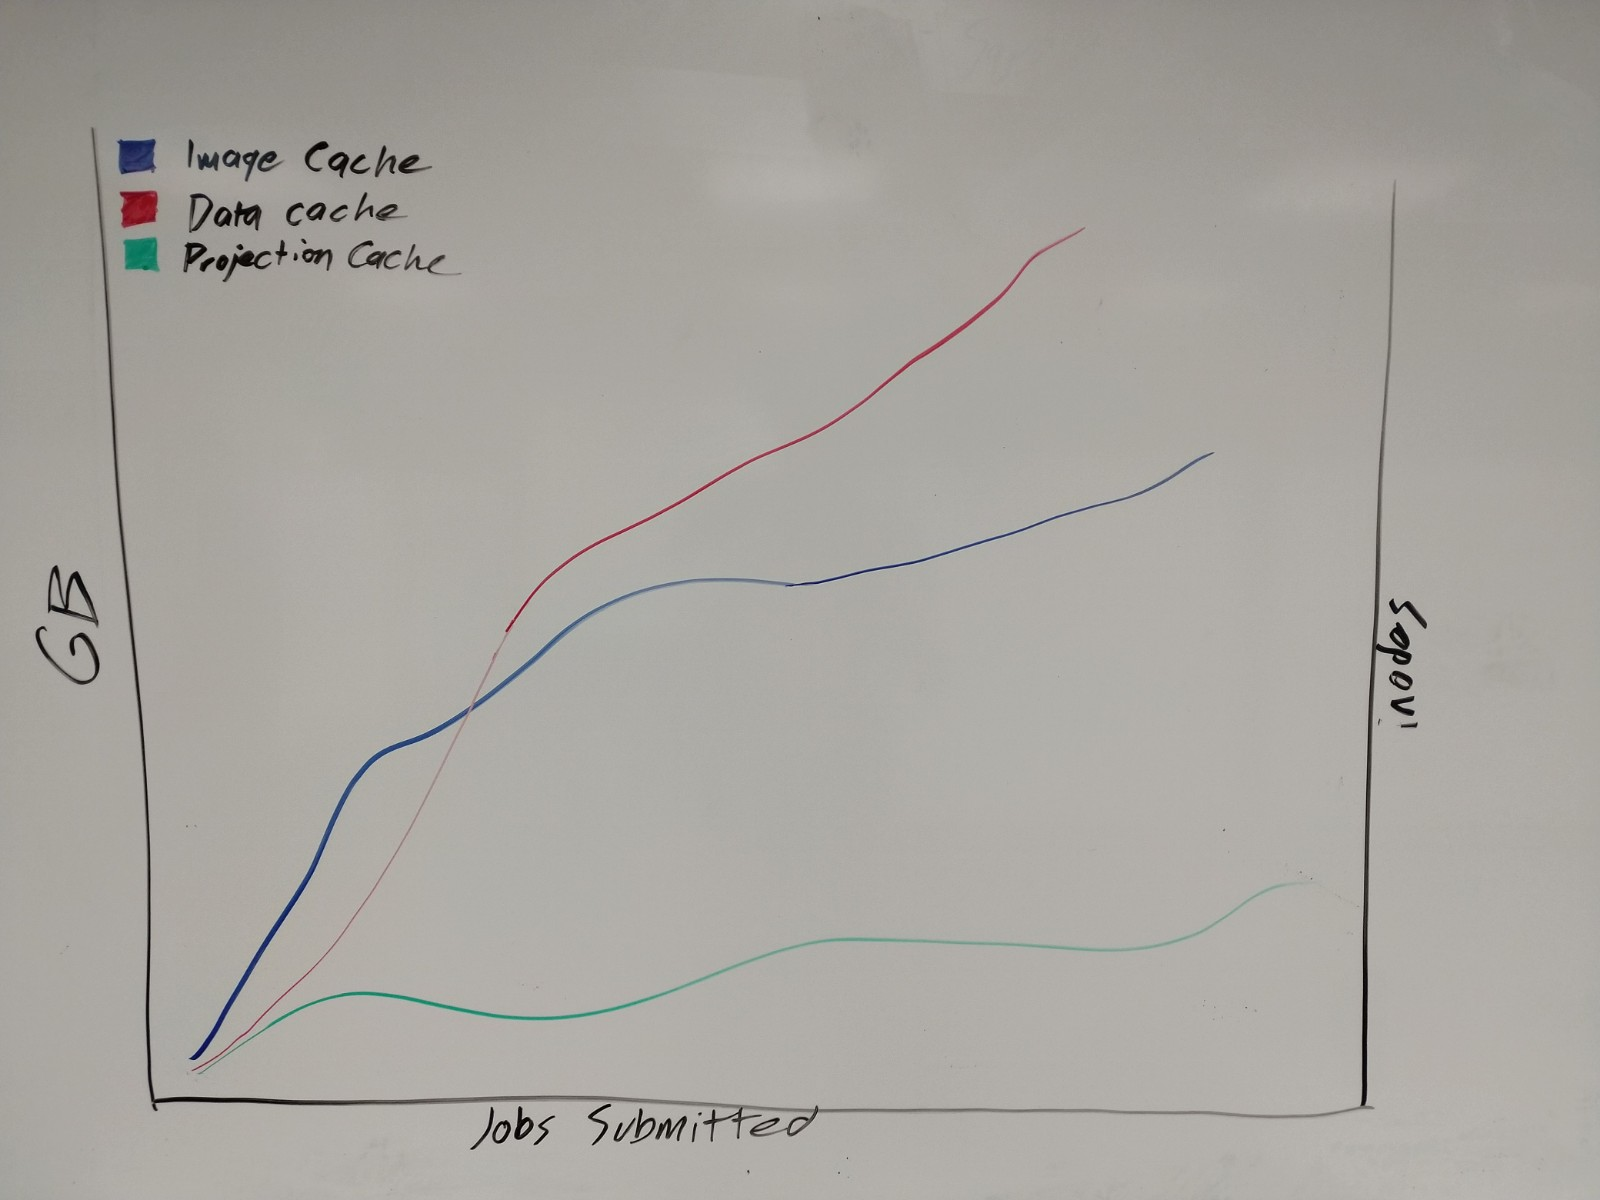
\includegraphics[width=\linewidth]{plots/IMG_20181116_101907.jpg}
\caption{Data and metadata costs with $\alpha=B$}
\end{figure}

\begin{figure}
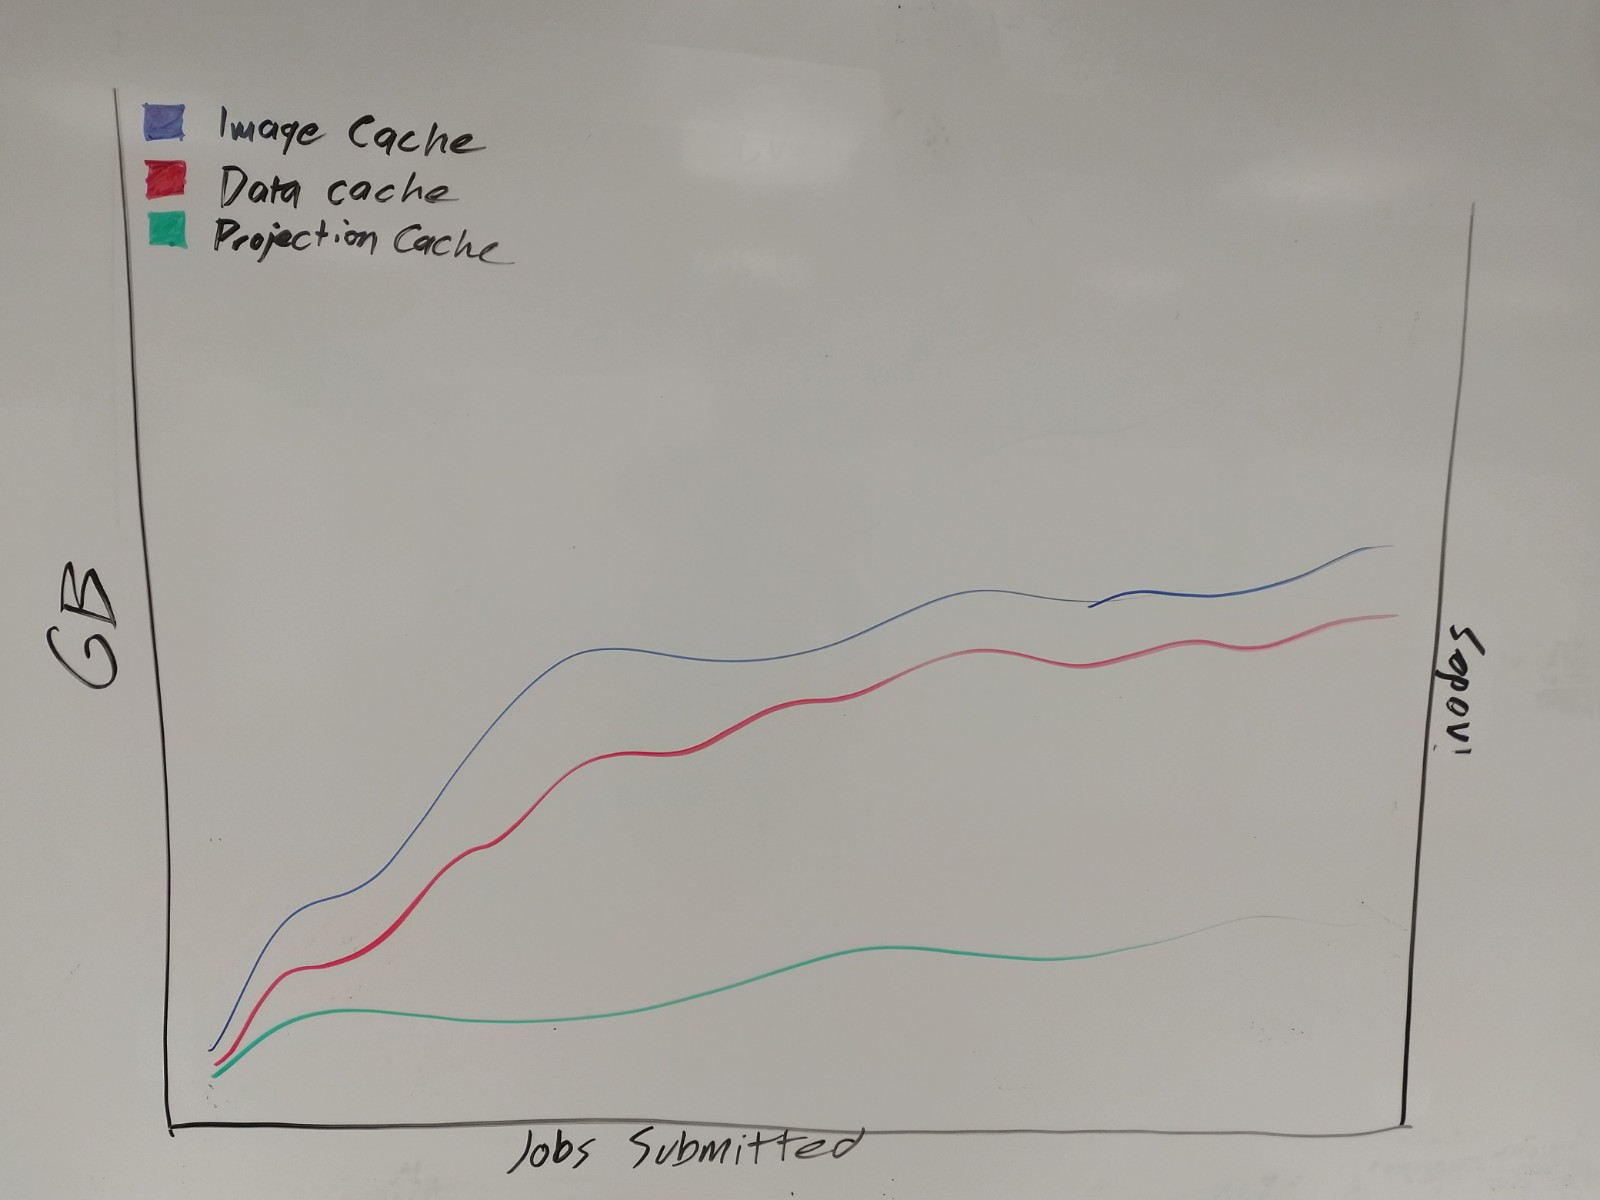
\includegraphics[width=\linewidth]{plots/IMG_20181116_102111.jpg}
\caption{Data and metadata costs with $\alpha=C$}
\end{figure}

\begin{figure}
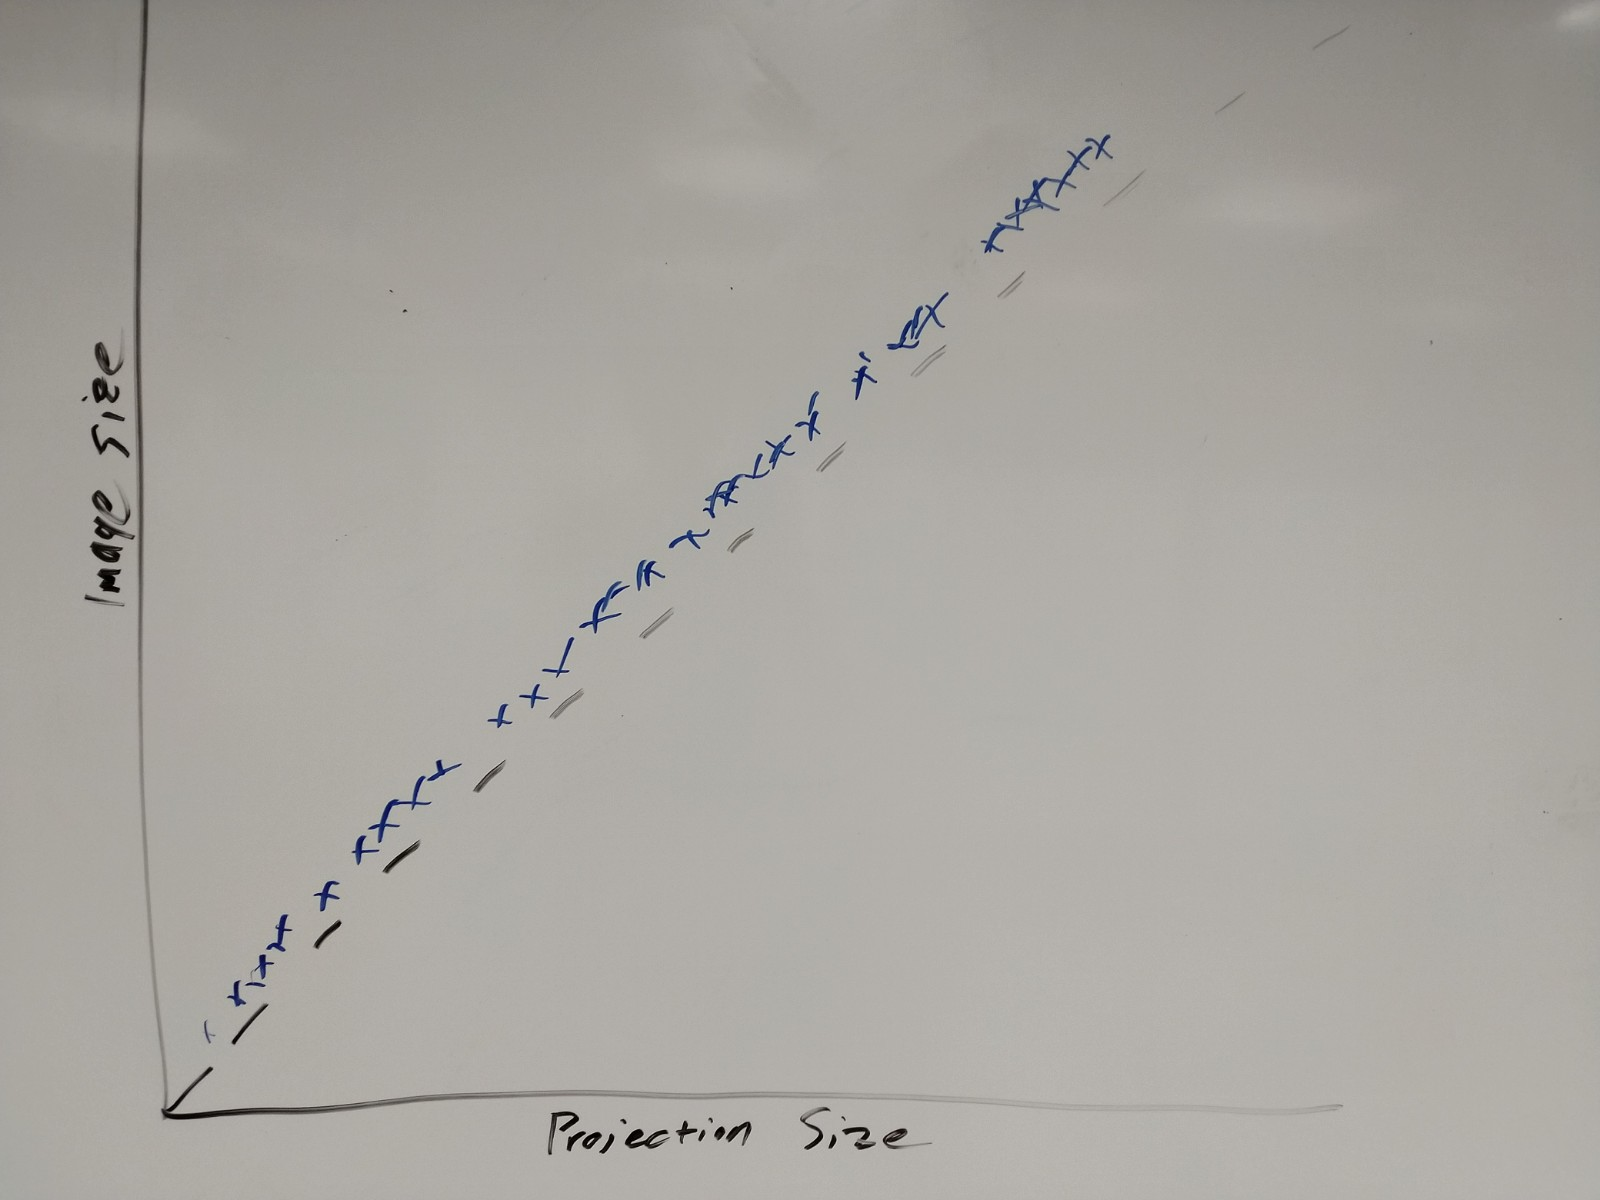
\includegraphics[width=\linewidth]{plots/IMG_20181116_102506.jpg}
\caption{Image size vs. requested projection size with $\alpha=A$}
\end{figure}

\begin{figure}
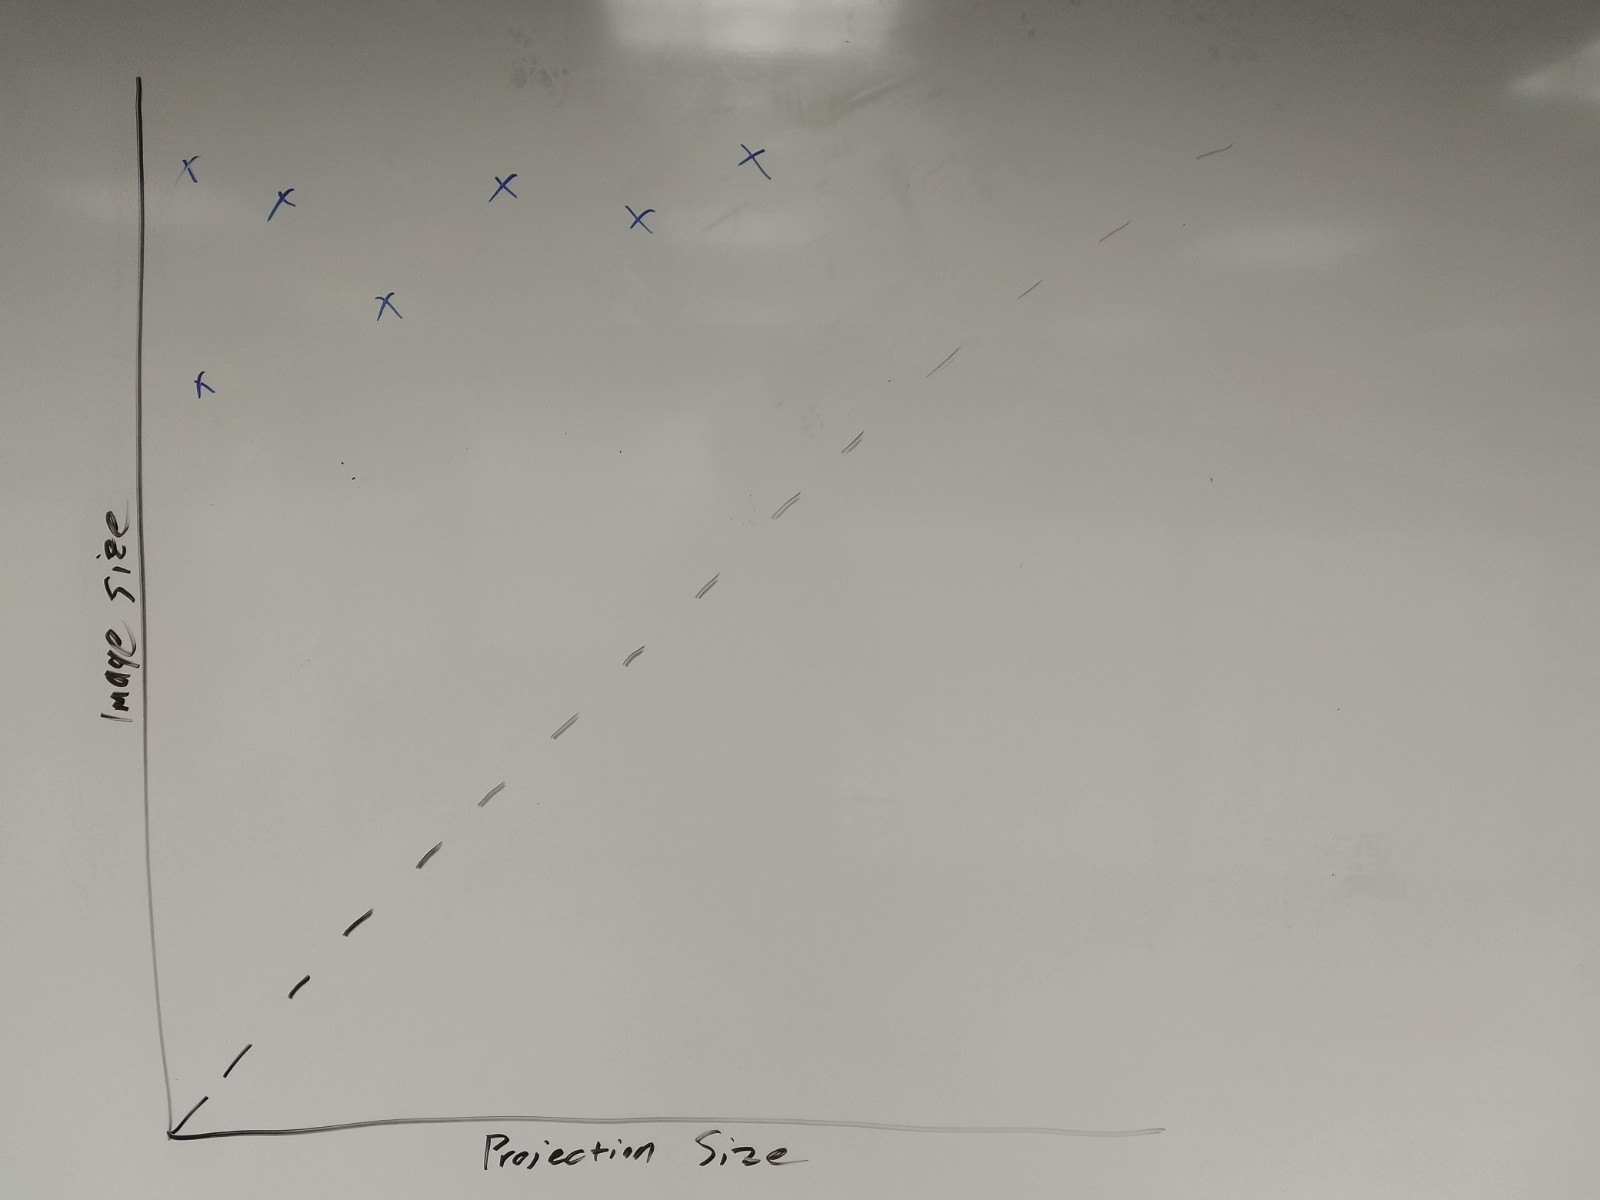
\includegraphics[width=\linewidth]{plots/IMG_20181116_102623.jpg}
\caption{Image size vs. requested projection size with $\alpha=B$}
\end{figure}

\begin{figure}
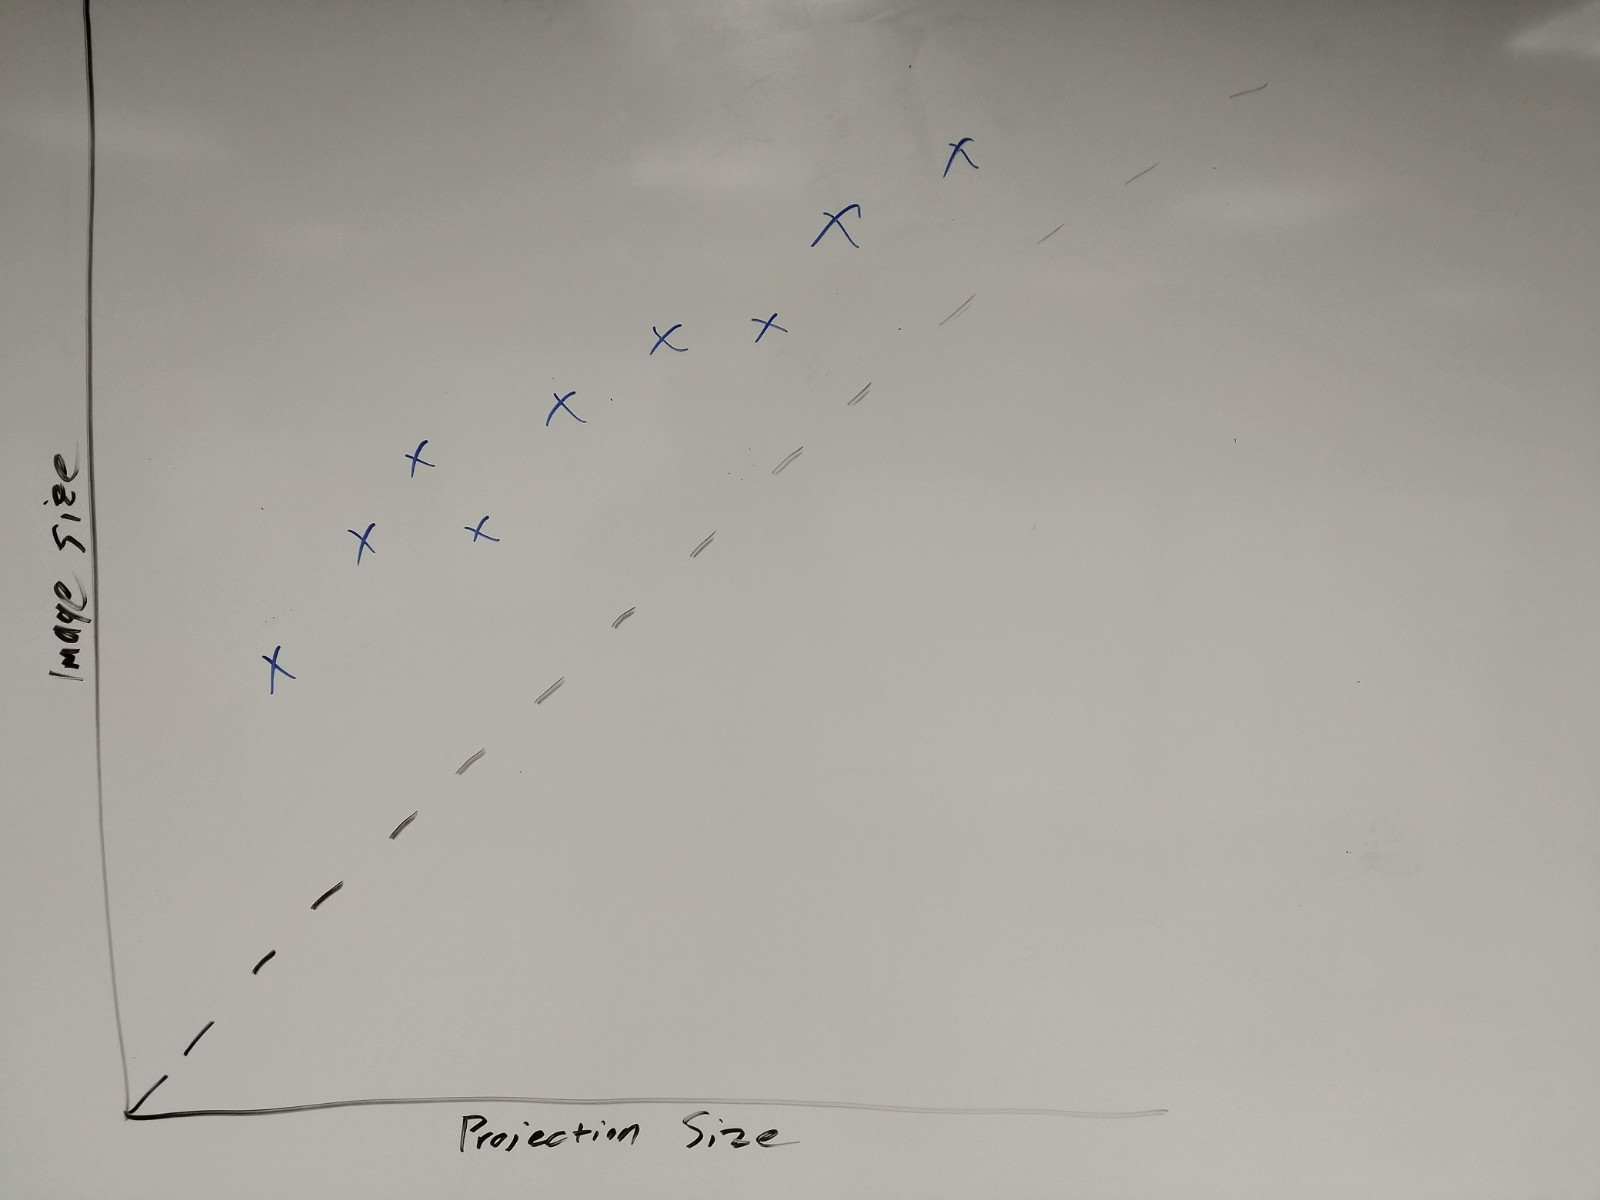
\includegraphics[width=\linewidth]{plots/IMG_20181116_102706.jpg}
\caption{Image size vs. requested projection size with $\alpha=C$}
\end{figure}

We implemented the pipeline described in section ?? on a cluster of RR machines at the Center for Research Computing~(CRC),
a high-performance computing site at the University of Notre Dame.
\Cref{tab:exp-setup} details the provisioned resources used in this test.
We used the sequence of jobs from WLCG submission log discussed in section ?? as a realistic source of events for our evaluation.
For each submission,
we used the simplified pipeline from section ?? to build an image for running each job.
We recorded the sizes of the image cache, projections, and data cache over the course of the workload.
Figure ?? shows the data and metadata costs observed.
We indeed observed rapid growth of the image cache with much slower increase in the underlying data cache.
Figure ?? shows the amount of time spent preparing images versus the size of the requested projection.
We see that preparation time is strongly correlated with the amount of data involved.

Next, we repeated this analysis using the projection pipeline described in section ?? and $\alpha = ??$.
We chose these values to illustrate the effects of extreme values as well as one we consider to be a good choice.
The results with $\alpha = W$ are very similar to those of the simplified pipeline.
This is to be expected,
since setting $\alpha$ to be very low limits the amount of merging performed.
Setting $\alpha = 0$ would approximate the simplified pipeline,
in that little to no merging occurs.

With $\alpha = X$,
projections were merged very frequently.
Figure ?? shows the steady increase in image size under this configuration.
We see a corresponding increase in time spent constructing images in figure ??.
With $\alpha$ set this high,
the time spent searching for a compatible image becomes much more significant,
hence the super-linear increase in build time.
Approximate Jaccard distance is extremely fast to compute in memory via MinHash without interacting with the filesystem.
As $\alpha$ is increased,
there is less filtering from this fast approximation.
Additional time is spent while Shrinkwrap walks the filesystem on a larger number of candidate images.
For very homogeneous workloads,
choice of $\alpha$ has less impact.
In this case, however,
different jobs are often incompatible with each other,
so eagerly merging projections resulted in poorly chosen combinations that prevented better fits in the future.
Thus we observe that the character of the workload is important in choosing $\alpha$.

Figures ?? and ?? show the same space and time costs, respectively,
as previously discussed for $\alpha = X$.
Here we note a much less pronounced increase in image storage cost than figure ??.
The increase in construction time is also less pronounced than in figure ??.
We chose this value of $\alpha$ to be more selective than Y to avoid ballooning images but still allow more merging than Z.
It is difficult to suggest values of $\alpha$ suitable for all cases since the machine configuration, workload, etc. all affect the patterns of behavior.
Based on experience,
we have found $\alpha$ values in the range V-W to be acceptable across a number of workloads and configurations.

\begin{table}
\centering
\begin{tabular}{c|c c}
& Cache Life (jobs) & Reuse count \\ \hline
$\alpha=a$ & small & small? \\
$\alpha=b$ & big & big \\
$\alpha=c$ & small? & big \\
\end{tabular}
\caption{Median cache life and number of reuses for container images}
\label{tab:cachelife}
\end{table}

We also measured the number of times a projection was reused or modified and how long images remained in the cache in an effort to estimate the reusability and relevance of images.
\Cref{tab:cachelife} tabulates these results.
With $\alpha = P$,
images were not reused as often as with the other values.
We suspect that this is because eager and frequent merges resulted in large images that were often incompatible with new jobs,
and that drifted away such that they were no longer close enough to any projection to be used.
The Jaccard distance metric penalizes elements in one set but not the other,
so as more and more projections are merged,
the resulting conglomerate moves farther and farther away from any single projection.
Eventually, it will fall out of use and age out of the cache.

In the other direction,
the simplified pipeline and $\alpha = Q$ also had many short-lived images.
This is likely because new images were often/always created for jobs,
so there was little reuse.
Due to the large number of images being created,
images were pushed out of the cache very frequently.

As part of the choice of $\alpha = Z$,
we tried to maximize the amount of reuse and image lifetimes.
This has the effect of indirectly minimizing storage and image construction time.
These are also very easy metrics to track as part of batch submission.
As such, they provide a simple way for administrators to optimize $\alpha$ to fit the system or workload.
Some manual tuning of this form is likely necessary for applying this sort of projection pipeline in situations significantly different from our test setup.

\section{Related Work}

\section{Conclusion}

\section{Reproducibility Data}

In an effort to provide consistent, reproducible results outlined are the
resources utilized in this paper and where they can be found.
Specific commits are mentioned to provide the exact version that was used.


All of these repositories are open source and contain Makefiles
and instructions on how to build and run them.

\section*{Acknowledgment}


\bibliographystyle{IEEEtran}
\bibliography{otherpapers,cclpapers}

\end{document}
